\documentclass[12pt,a4paper]{report}
\usepackage{graphicx}
\usepackage[utf8]{inputenc}
\usepackage[T1]{fontenc}
\usepackage[a4paper,top=3cm,bottom=2cm,left=3cm,right=3cm,marginparwidth=1.75cm]{geometry}
\usepackage[spanish]{babel}
\selectlanguage{spanish}
\usepackage{fancyhdr}

% quitar el 0.
\renewcommand\thesection{\arabic{section}}

% aqui definimos el encabezado de las paginas pares e impares.
\lhead[x1]{
\includegraphics[width=1cm]{./images/epis}}
\chead[y1]{}
\rhead[z1]{Inteligencia de Negocios}
\renewcommand{\headrulewidth}{1pt}

% aqui definimos el pie de pagina de las paginas pares e impares.
\lfoot[a1]{Ing. Patric Cuadros}
\cfoot[c1]{}
\rfoot[e1]{\thepage}
\renewcommand{\footrulewidth}{1pt}

\pagestyle{fancy} 



\begin{document}
\begin{titlepage}
	\centering
	
\includegraphics[width=4cm]{./images/upt}\par\vspace{1cm}
	{\scshape\LARGE\huge\bfseries Universidad Privada de Tacna \par}
	{\scshape\LARGE Escuela de Ingenieria de Sistemas \par}
	\vspace{1cm}
	{\scshape\Large Inteligencia de Negocios\par}
	\vspace{0.5cm}
	{\huge\bfseries Diseño de Indicadores ICACIT\par}
	\vspace{1cm}

	{\Large\itshape PRESENTADO POR:\par}
	{\Large\itshape Gary Calle Cortez (2013000664)\par}
	{\Large\itshape Aldo Lopez Mamani\par}
	{\Large\itshape Renzo Moreno\par}
	{\Large\itshape Christian Cespedes Medina\par}
	{\Large\itshape Tommy Morales\par}
	{\Large\itshape Leonardo Acevedo Vasquez\par}

	\vfill
	Docente\par
	Ing. Patrick Cuadros\textsc{Brown}

	\vfill

% Bottom of the page
	{\large \today\par}

\end{titlepage}

%% Aquí podemos añadir un resumen del trabajo (o del artículo en su caso) 
\begin{abstract}
El siguiente informe trata sobre los criterios de ICACIT estableciendo los indicadores para Condicion o Criterio ,determinacion de el Área Responsable de los indicadores y una posible consulta en SQL que ingeste este indicador.
\end{abstract}

%% Iniciamos "secciones" que servirán como subtítulos
%% Nota que hay otra manera de añadir acentos


\addcontentsline{toc}{chapter}{Índice general}
\tableofcontents
\newpage

\begin{Large}
\textbf{INDICADORES} 
\end{Large}
\section{Criterio estudiantes}

\subsection{Evaluacion del desempeño y monitoreo del progreso de los estudiantes}
Un indicador visible es el cumplimiento de los PRE-REQUISITOS, esto de analiza con los cursos que presenten pre-requisitos dentro de la base de datos y la aprobacion de estos dentro de los cursos aprobados por cada estudiante
\begin{itemize}
\item Area encargada: Matricula

\end{itemize}
\subsection{Consejería de Estudiantes}
Un indicador visible es la frecuencia en que los estudiantes acuden a consejeria estudiantil, esto se podra corroborar en la base de datos con su registro al acudir a este servicio
\begin{itemize}
\item Area encargada: Tutoria

\end{itemize}
\subsection{Traslado de Estudiantes y Transferencia de Cursos}
Un indicador visible son la procedencia de los traslados, todos los requisitos y datos del traslado como su procedencia, pais o departamente es un indicador de donde generalmente solicitan dichos traslados y toda esa dato se almacena en la base de datos
\begin{itemize}
\item Area encargada: Matricula

\end{itemize}
\subsection{Requisitos de Graduación}
Un indicador visible son los requisitos para la graduacion como el numero de creditos, horas de practicas pre-profesionales, en donde solicitaron las practicas o si varios egresados la hacen regularmente en algun estatal o privado, los datos de el grado del nuevo ingeniero de sistemas se almacenan en distintas tablas relacionadas
\begin{itemize}
\item Area encargada: Egresados

\end{itemize}

\section{ Criterio Objetivos educacionales del programa}
\textbf{2.1 Indicadores }\\

Condicion: Tener objetivos educacionales consistentes con la mision de la institucion.\\

\textbf{2.2 Area responsable}\\

Escuela profesional de ingenieria de sistemas\\
Vicerrectorado Academico\\

\textbf{2.1 Consulta SQL}\\

SELECT objetivos\_institucionales, escuelta\_profesional FORM objetivos WHERE escuela\_profesional = 'EPIS'

\section{ Criterio resultados del estudiante}
\textbf{3.1 Indicadores para Condición o Criterio}
\begin{center}
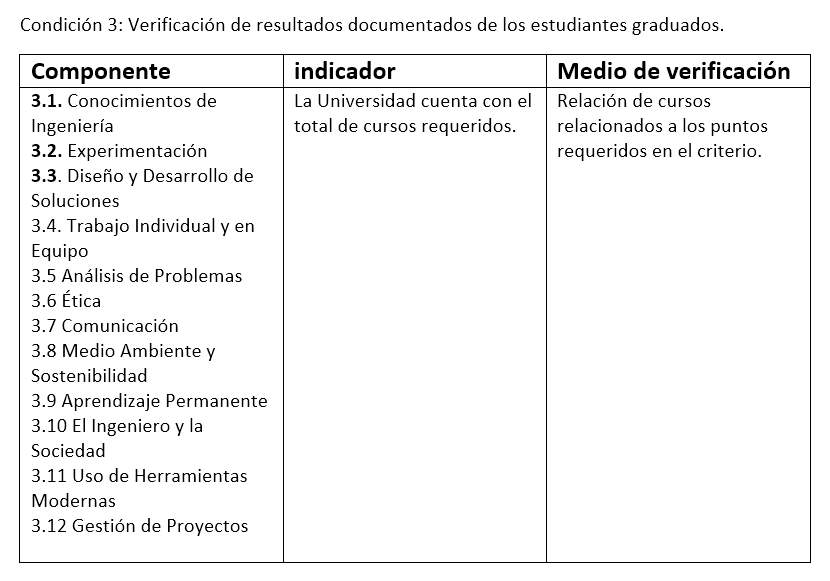
\includegraphics[width=15cm]{./Images/resultado}
\end{center}	

\textbf{3.2 Área Responsable de este Indicador}

 Area: Facultad de Ingeniría de Sistemas

\textbf{3.3 Consulta posible en SQL que ingeste este indicador}\\

SELECT dpto,facultad,nombre\_asignatura FROM programas INNER JOIN asignaturas ON programas.nombre\_facultad = asignatura.id\_asignatura


\section{ Criterio mejora continua}
La mejora continua es un proceso de evolución del estado actual de un proceso, en este caso el de enseñanza. Nuevas teorías y practicas son publicadas constantemente por lo que no debemos quedarnos estancados, debemos buscar adaptarnos a estos cambios ya que estos cambios son para llegar a ser mejores ingenieros.

\begin{itemize}
\item Área Encargada: Docentes, Egresados.
\item Query: SELECT eg.nombre,su.sugerencia FROM egresados eg INNER JOIN sugerencia su ON eg.id = su.egresadoid
Esta consulta se basa en que en la reunión de docentes y egresados, los docentes les preguntan a los egresados que les sirvió mas de lo aprendido en la universidad y que les falto según su experiencia laboral.
\end{itemize}

\section{ Criterio plan de estudios}
El plan de estudio debe especificar áreas temáticas apropiadas para la ingenería e incluir un año de una combinación de \textbf{Matemática de nivel Universitario} y \textbf{Ciencias Básicas}, un año y medio \textbf{Tópicos de Ingeniería} y \textbf{Diseño en ingenería}.

\begin{itemize}
\item Area encargada: Facultad de Ingeniería

\item Posible Consulta: Una consulta o revisión en los cursos que ofrece la universidad donde Matemáticas de Nivel Universitario: Matemáticas por encima del nivel de pre-cálculo
Ciencias Básicas: Consisten en química y física, y otras ciencias naturales incluyendo las ciencias de la vida, de la tierra y espaciales.\\
Diseño en Ingeniería: Proceso creativo, iterativo y de toma de decisiones, en el que las ciencias básicas, las matemáticas y las ciencias de la ingeniería son aplicadas para buscar soluciones viables a un problema que no necesariamente tiene una única respuesta.\\
Select nombre From Cursos where tipo = ING

\item Tabla Involucrada: Cursos
\end{itemize}

\section{ Criterio cuerpo de profesores}
El cuerpo de profesores es fundamental como parte de la enseñaza de una facultad de la universidad, los integrantes de este grupo son buscados o seleccionados mediante un examen para proveer el mejor servicio posible.

\begin{itemize}
\item Area encargada: Facultad de Ingeniería

\item Query: SELECT fa.nombre, docente.nombre FROM docentes do INNER JOIN facultadad fa ON fa.idfacultad = do.idfacultad. Esta consulta nos devolvera todos los nombres de los docentes y la facultad a la que pertenecen.

\item Tabla Involucrada: Docente, Facultad.
\end{itemize}

\section{ Oficinas, Salas de Clase y Laboratorios}
\subsection{Evaluacion del desempeño y monitoreo del progreso de los estudiantes}
Un indicador visible es la realizacion de inventariado de los inmuebles, agrando datos como marca, color, fecha de adquisicion, etc.
cada salon de clases esta asociado a distintos equipos como proyectores, ordenadores camaras de seguridad o servidores, ese indicador es muy util
Hay un inidcador mucho mas importante ya que es la realizacion del inventariado y asociacion de las distintas computadoras, servidores con los laboratorios asi mismo con la composicion del hardware de cada implemento

\begin{itemize}
\item Area encargada: Almacen, Asignacion de recursos y seguridad

\end{itemize}
\subsection{Guía y Orientación}
Un indicador que se renova todos los ciclos es la capacitacion tanto de docentes y alumnos en el uso correcto de las intalacions y aula vitual, esto se da en los primeros ciclos y corroborando la asistencia de dichos alumnos y docentes de manera obligatoria

\begin{itemize}
\item Area encargada: Capacitacion

\end{itemize}
\subsection{Servicios de Biblioteca}
Es un claro indicador de la frecuencia de usos de los distintos libros, dependiendo de su area (salud, derecho, ingenieria, etc) y la cantidad que son solicitados, esto podra indicar que tipo de libros son mas requeridos constantemente tanto por docentes o estudiantes y que libros no son tan solicitados.

\begin{itemize}
\item Area encargada: Biblioteca, Almacen

\end{itemize}
\subsection{Recursos Informáticos }
Hay un indicador del tipo de ordenadores y servidores que son utilizados por los alumnos,  asi como los sistemas operativos adecuados y los softwares instalados legalmente

\begin{itemize}
\item Area encargada: Almacen, Asignacion de recursos, seguridad y TI

\end{itemize}

\section{ Criterio apoyo institucional}
Criterio referido al apoyo brindado a cierto grupo de personas de pocos recursos para asistir a su carrera deseada en una Universidad. De este criterio podemos saber quienes y cuantos cuantos estudiantes pertenecientes a este servicio hay por facultad y la carrera a la que pertenecen.

\begin{itemize}
\item Area encargada: Facultad de Ingeniería

\item Query: SELECT fa.nombre, es.nombre, ai.nombrealumnoi  FROM facultad fa INNER JOIN apoyoinstitucional ai ON fa.idfacultad = ai.idfacultad INNER JOIN escuela es ON fa.idfacultad = es.idfacultad. Con este query obtendremos todos los alumnos pertenecientes al servicio de apoyo con su respectiva facultad y escuela en la que estan.

\item Tabla Involucrada: Facultad, Escuela, Apoyo Institucional.
\end{itemize}

\section{ Criterio investigacion}
Este criterio se refiere a un grupo de investigacion de una facultad buscando mejorar ya sea el servicio brindado o participar en trabajos de investigacion nacionales y/o internacionales.

\begin{itemize}
\item Area encargada: Facultad de Ingeniería

\item Query: SELECT fa.nombre, in.nombremiembro FROM investigacion in INNER JOIN facultad fa ON in.idfacultad = fa.idfacultad. Con este query se busca saber todos los miembros del grupo de investigacion por facultad.

\item Tabla Involucrada: Investifacion, Facultad.
\end{itemize}

\end{document}
